\section*{Parallelization of Matrix-Vector Multiplication and the Power Method}

This report describes the code and result of designing and implementing an algorithm for finding the highest eigenvalue of a matrix, called the Power Method.  The algorithm is designed to run in parallel on N processors to enhance the performance. The Power Method  can easily be described by the following Matlab code 
\lstinputlisting[language=matlab, caption={Power Method algorithm implemented in Matlab (by John R. Gilbert)}]{./code/powermethod.m}

\subsection*{Implementation in the C language}
The code was implemented in C using the MPI library for parallelization. The design of the code was based on first partitioning the matrix operation between the N processors. First a matrix where generated in the function $generatematrix()$. This function generated $\frac{N}{nprocs}$ where nprocs is the number of processors. Further in the code each processors did operations on the same amount of rows. Further, following the algorithm in Listing 1, each processor generated a row column vector of dimension N with 1's in all the entries. Each processor executed the $norm2()$ function on the vector. The parallelization used that helped the performance the most where implemented in the matrix-vector multiplication, in the funciton matVec(). Each processor performed a multiplication with each of the rows and the column vector, producing a column vector of dimension $\frac{N}{nprocs}$. The column vectors from all the processors where gathered in processor 0 using the $MPI\_gather$ library function to form the total matrix-vector product $Ax$. To make the total vector accessible to the other processors, $MPI\_Bcast$ where used. For more details the reader should look at the c-code implementations in functions.c.

\subsection*{Performance and timing}
The c-code where tested on matrices of dimension $N$ where $N$ allways where the quotient $\frac{N}{nprocs}$ always was an integer. The algorithm proved successful and returned the same values as the matlab code, both using the matrix provided in the assignment text, and on an arbitrary matrix. For the timing of the code the dimension matrix dimension $N=2400$ where used, yielding 25.67 seconds of execution time running the code on one processor. The rest of the execution times can be found in Fig. 1 and Table 1. 

\begin{table}
\center
    \begin{tabular}{|l|l|}
        \hline
        nprocs & Execution Time (Seconds) \\ \hline
        1      & 25.67                    \\ 
        2      & 12.95                    \\ 
        4      & 6.47                     \\ 
        8      & 3.41                     \\ 
        16     & 1.97                     \\
        \hline
    \end{tabular}
\end{table}

\begin{figure}[h!] 
 \center 
 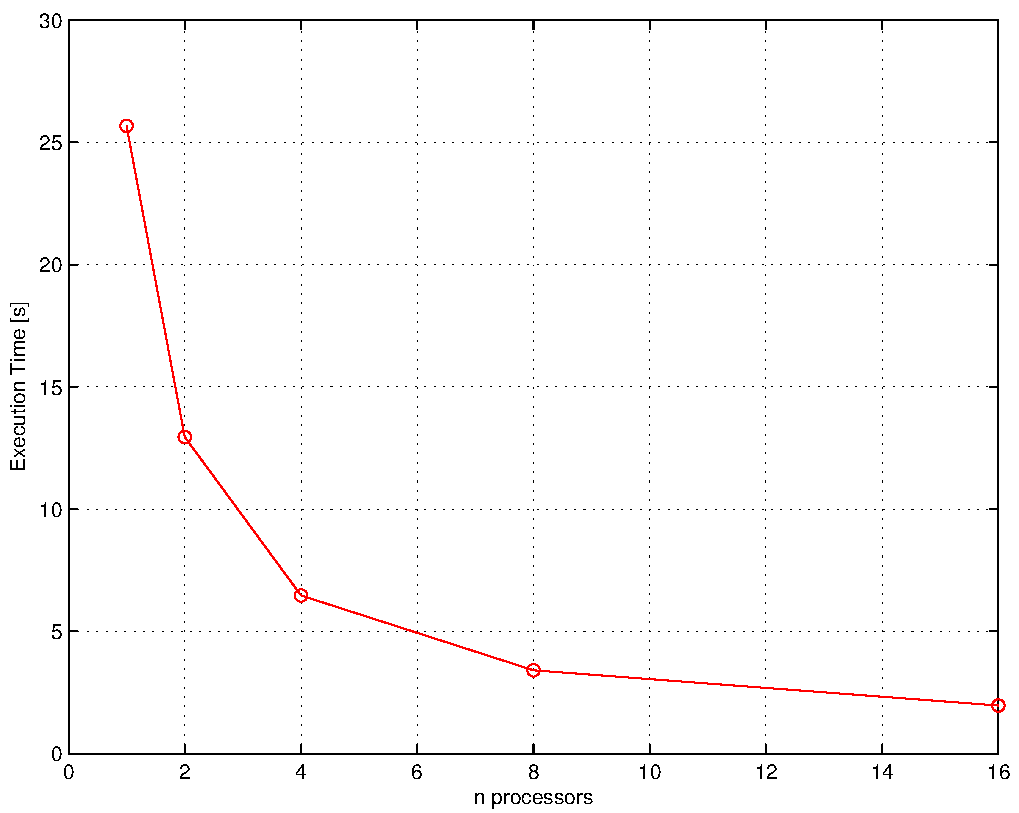
\includegraphics[scale=0.7]{./figures/plot1.pdf}
 \caption{ Plot of the execution times for the code running on 1 to 16 processors \label{fig:plot}}
 \end{figure}

\begin{figure}[h!] 
 \center 
 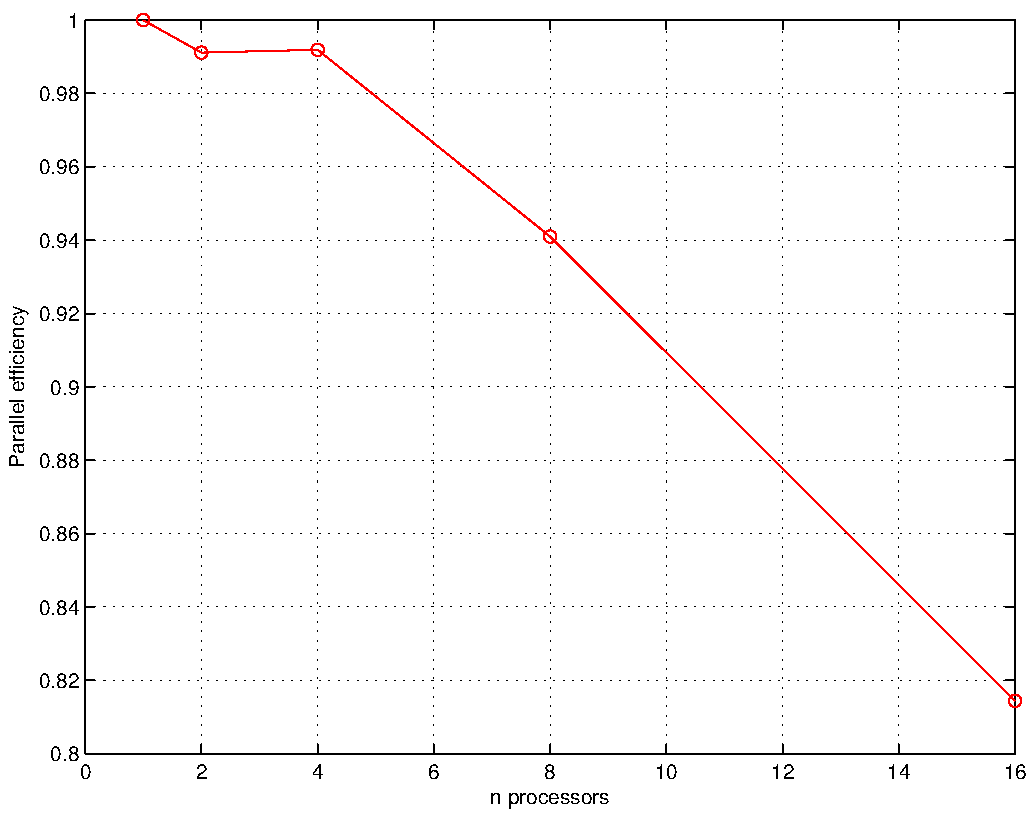
\includegraphics[scale=0.7]{./figures/plot2.pdf}
 \caption{  Plot of the parallel efficiency for the different numbers of processors\label{fig:para}}
 \end{figure}

As we can from Fig. \ref{fig:plot} and Fig. \ref{fig:para} the parallelization of the code worked very well. On matrices with high dimensions the execution time where almost halved when the number of processors where doubled, for a small number of processors. 

\subsection*{Tau Profiling Tool}
The Tau Profiling tool where used to analyze the performance of the code both with a text based interface and with the graphical interface $paraprof$. 

\begin{figure}[h!] 
 \center 
 \subfloat[]{ 
 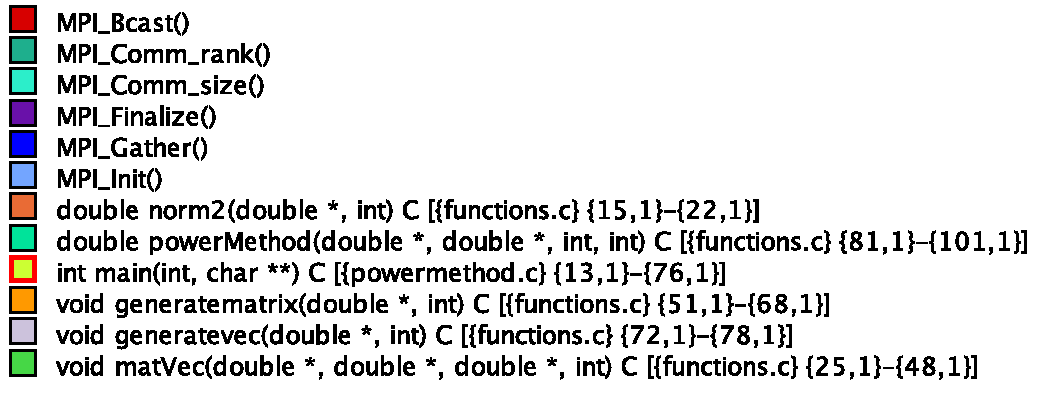
\includegraphics[scale=0.4]{./figures/legend_16.pdf} } \\
 \subfloat[]{ 
 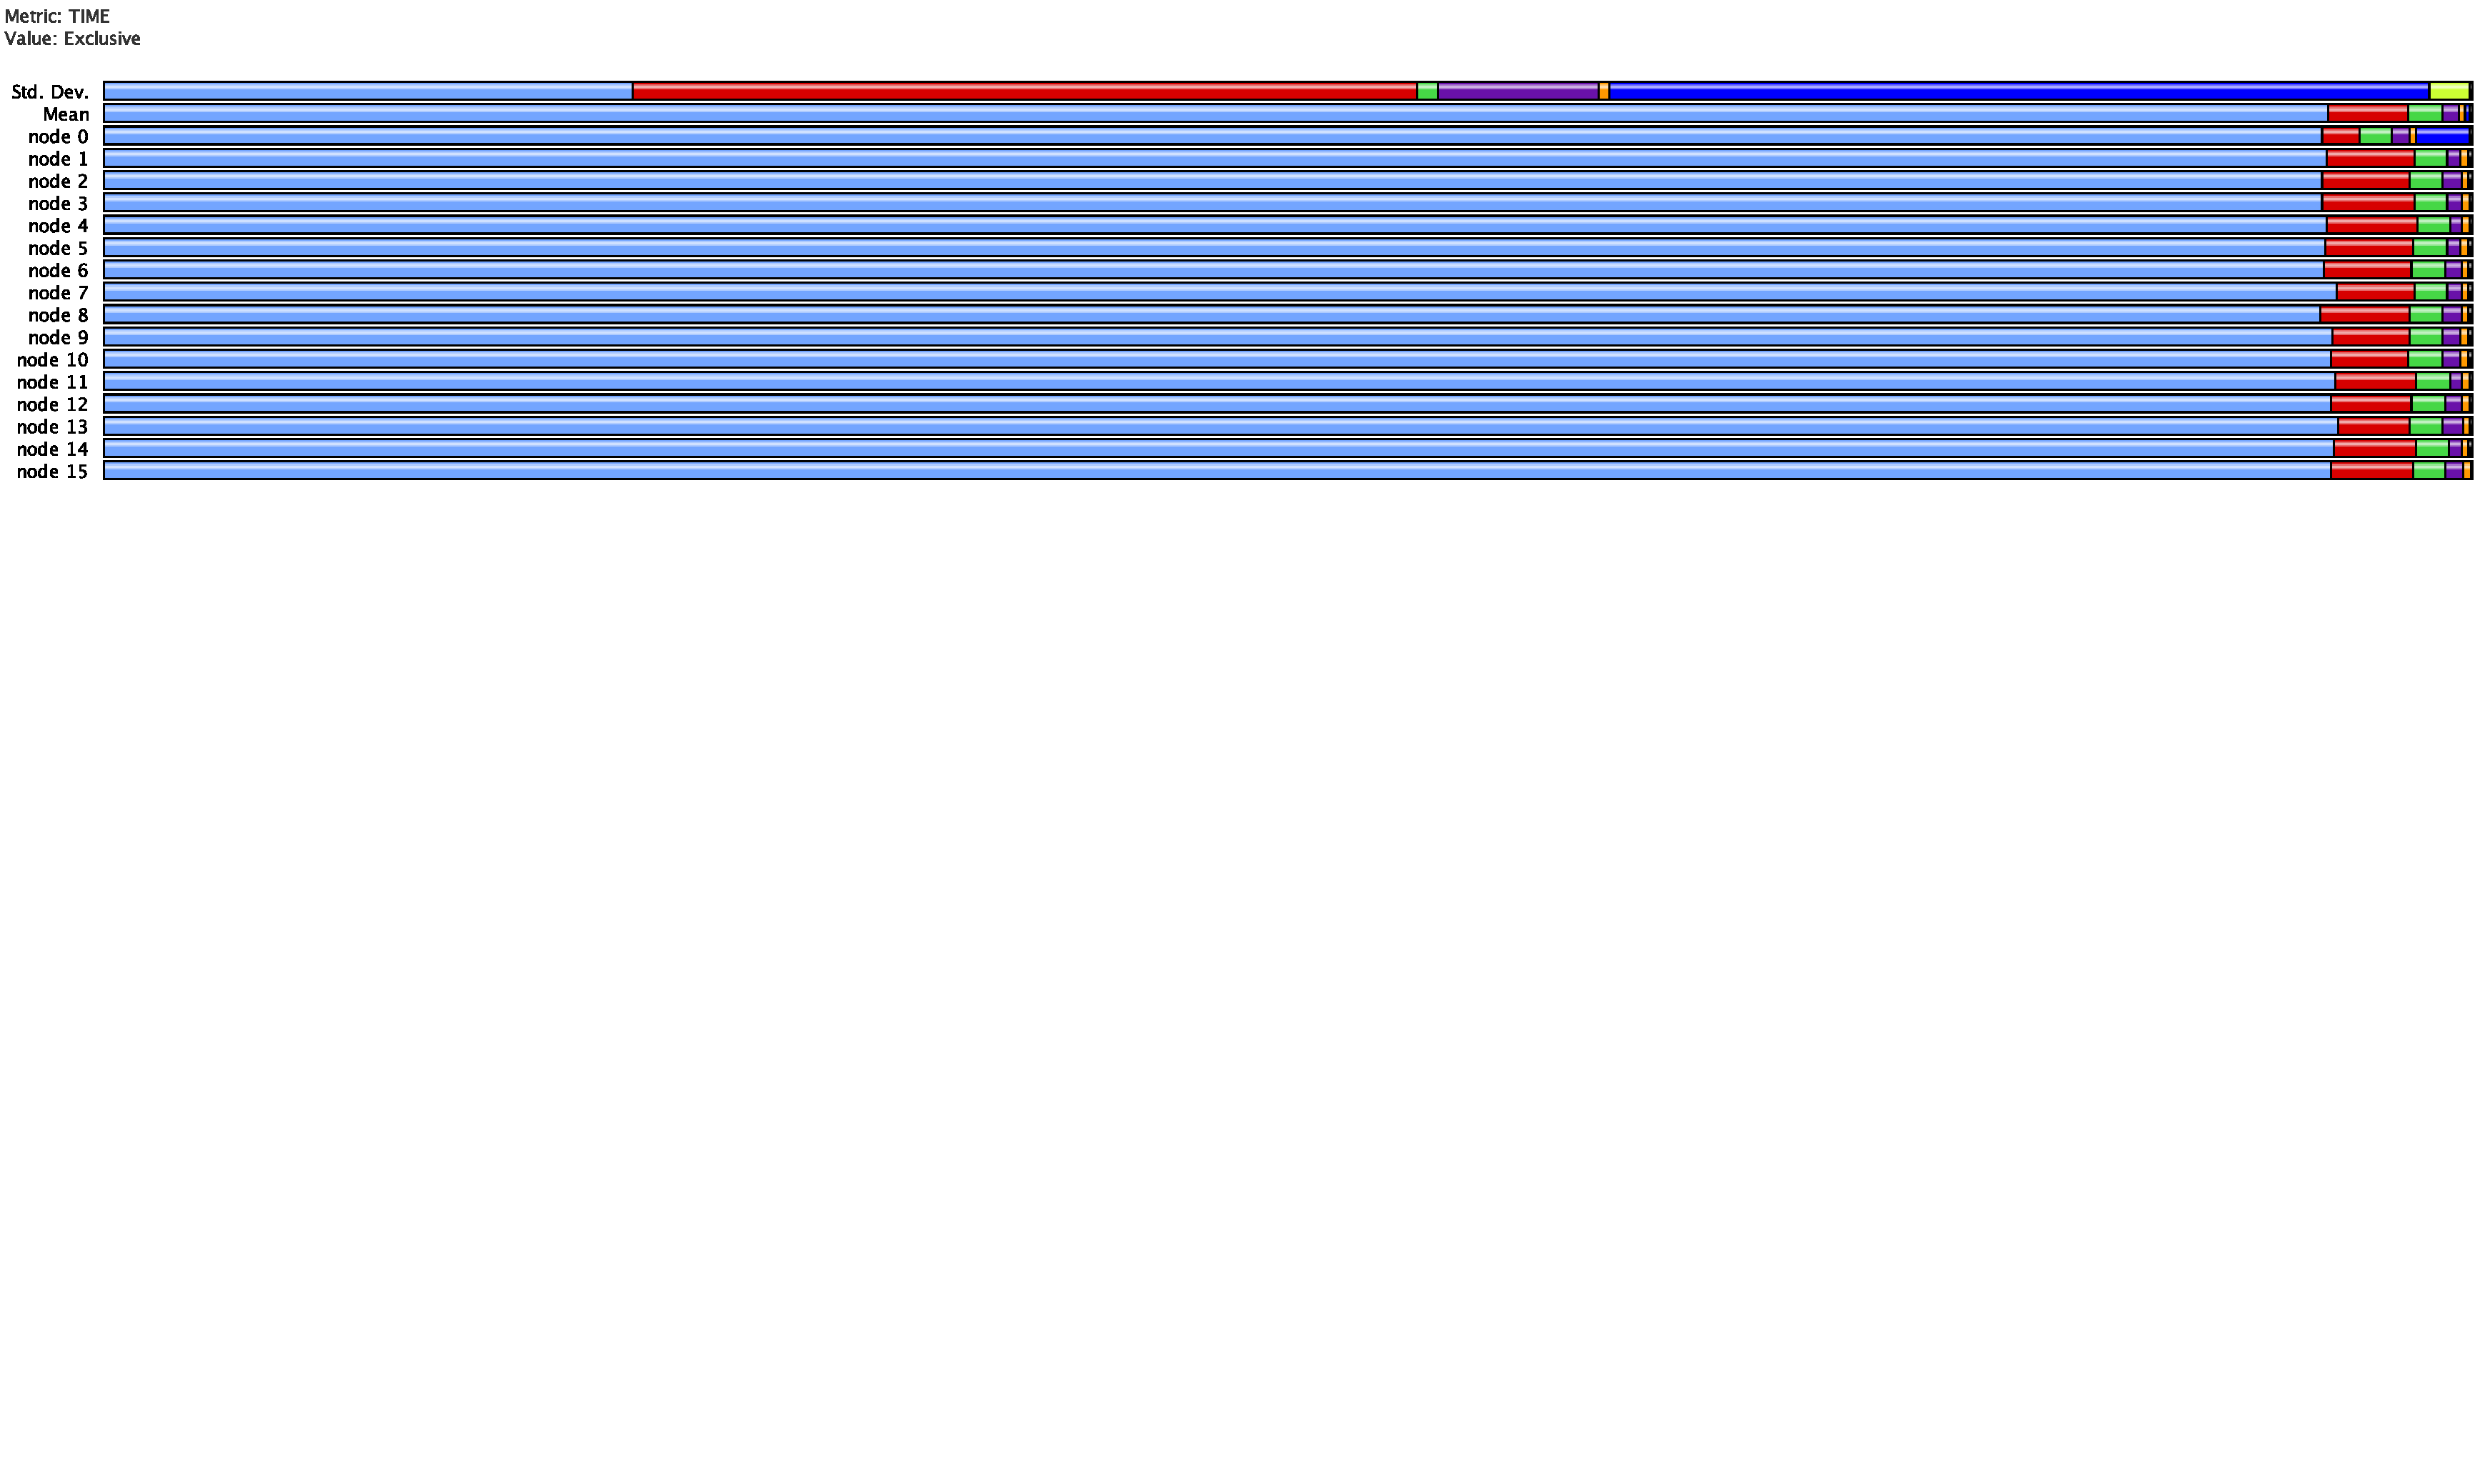
\includegraphics[scale=0.3]{./figures/paraprof_pic_16.pdf} }
 \caption{ The figure shows the execution time for the different MPI functions running on the different processors \label{fig:}}
 \end{figure}

\begin{figure}[h!] 
 \center 
 \subfloat[]{ 
 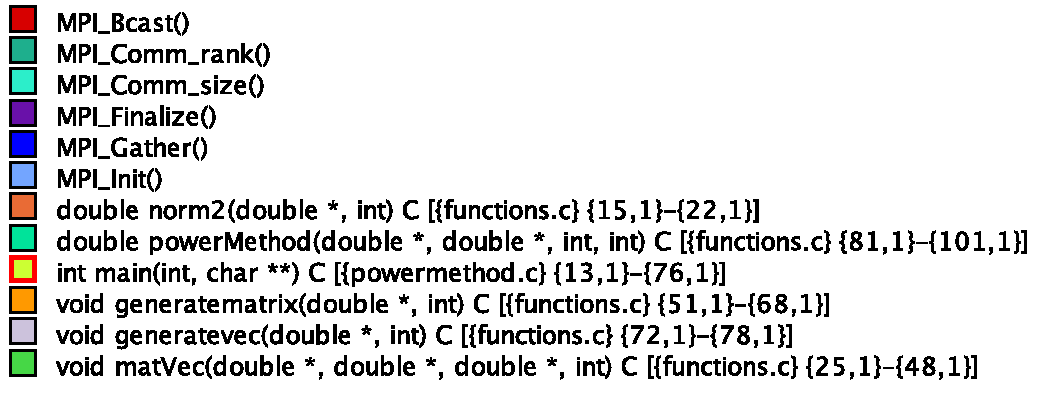
\includegraphics[scale=0.4]{./figures/legend_16_inclusive.pdf} } \\
 \subfloat[]{ 
 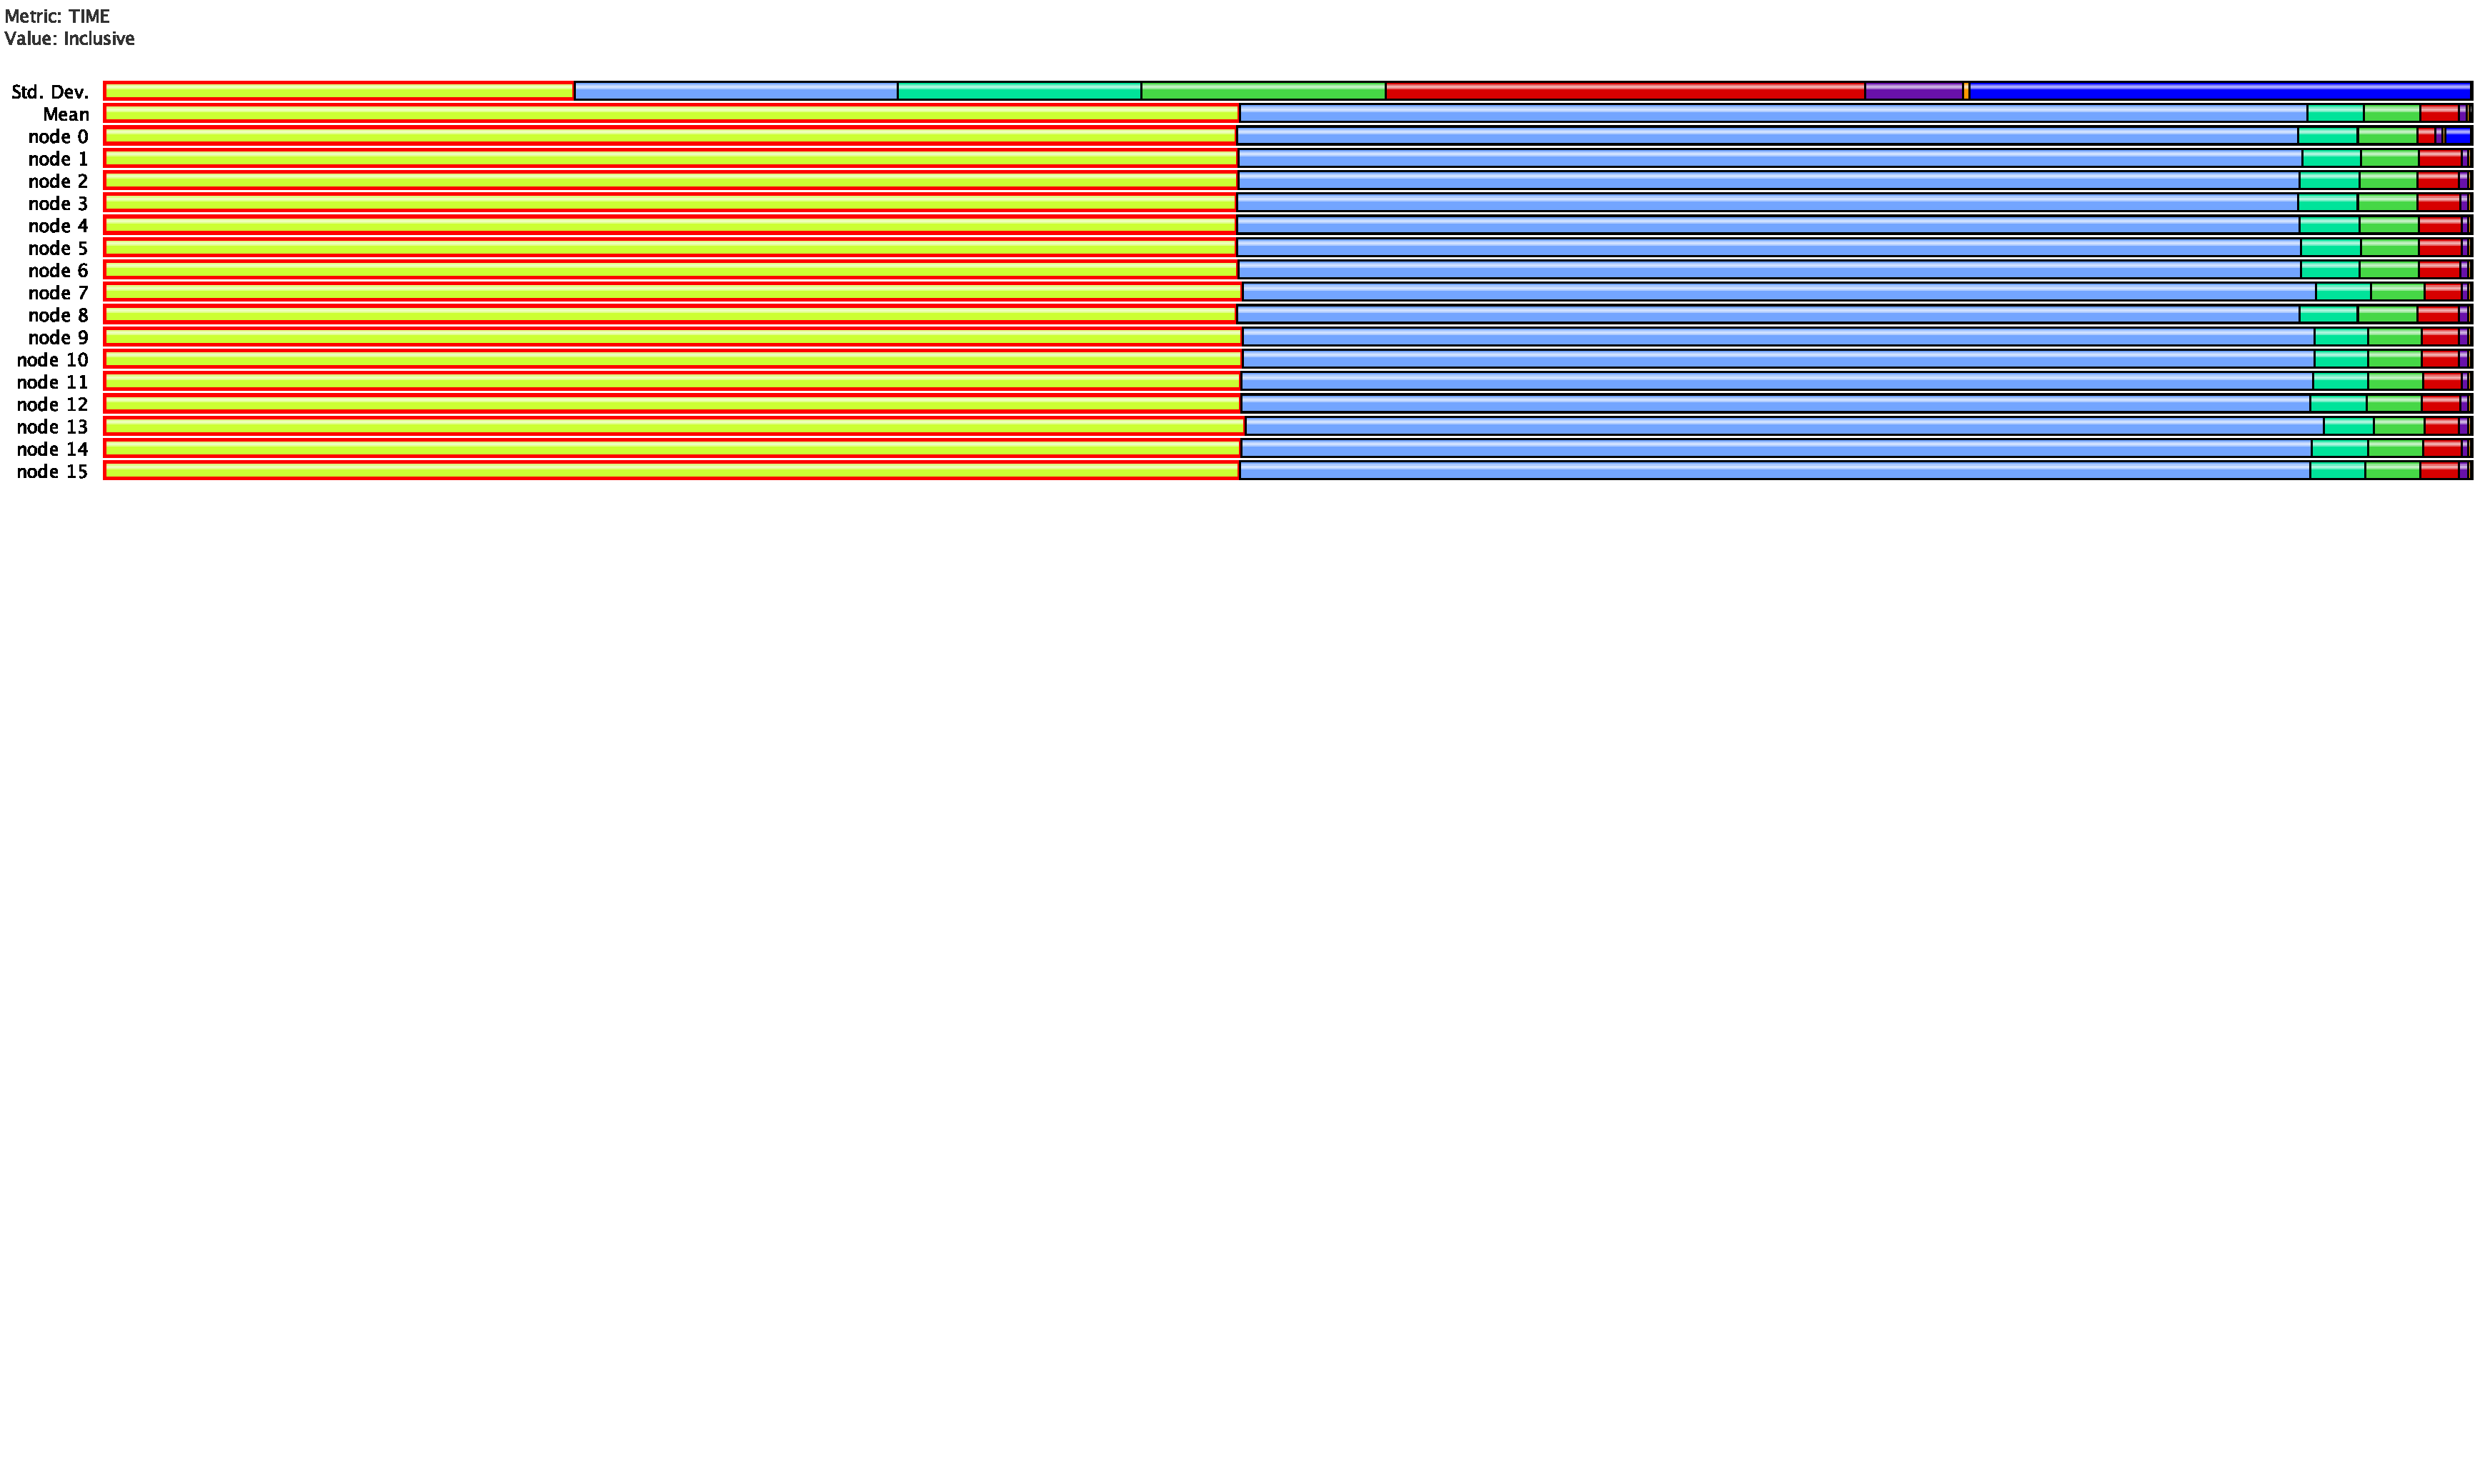
\includegraphics[scale=0.3]{./figures/paraprof_pic_16_inclusive.pdf} }
 \caption{ The figure shows the execution time for all the functions on the different processors \label{fig:}}
 \end{figure}

\clearpage


\appendix

\subsection*{A.1 pprof output}
\subsection*{4 Processors}


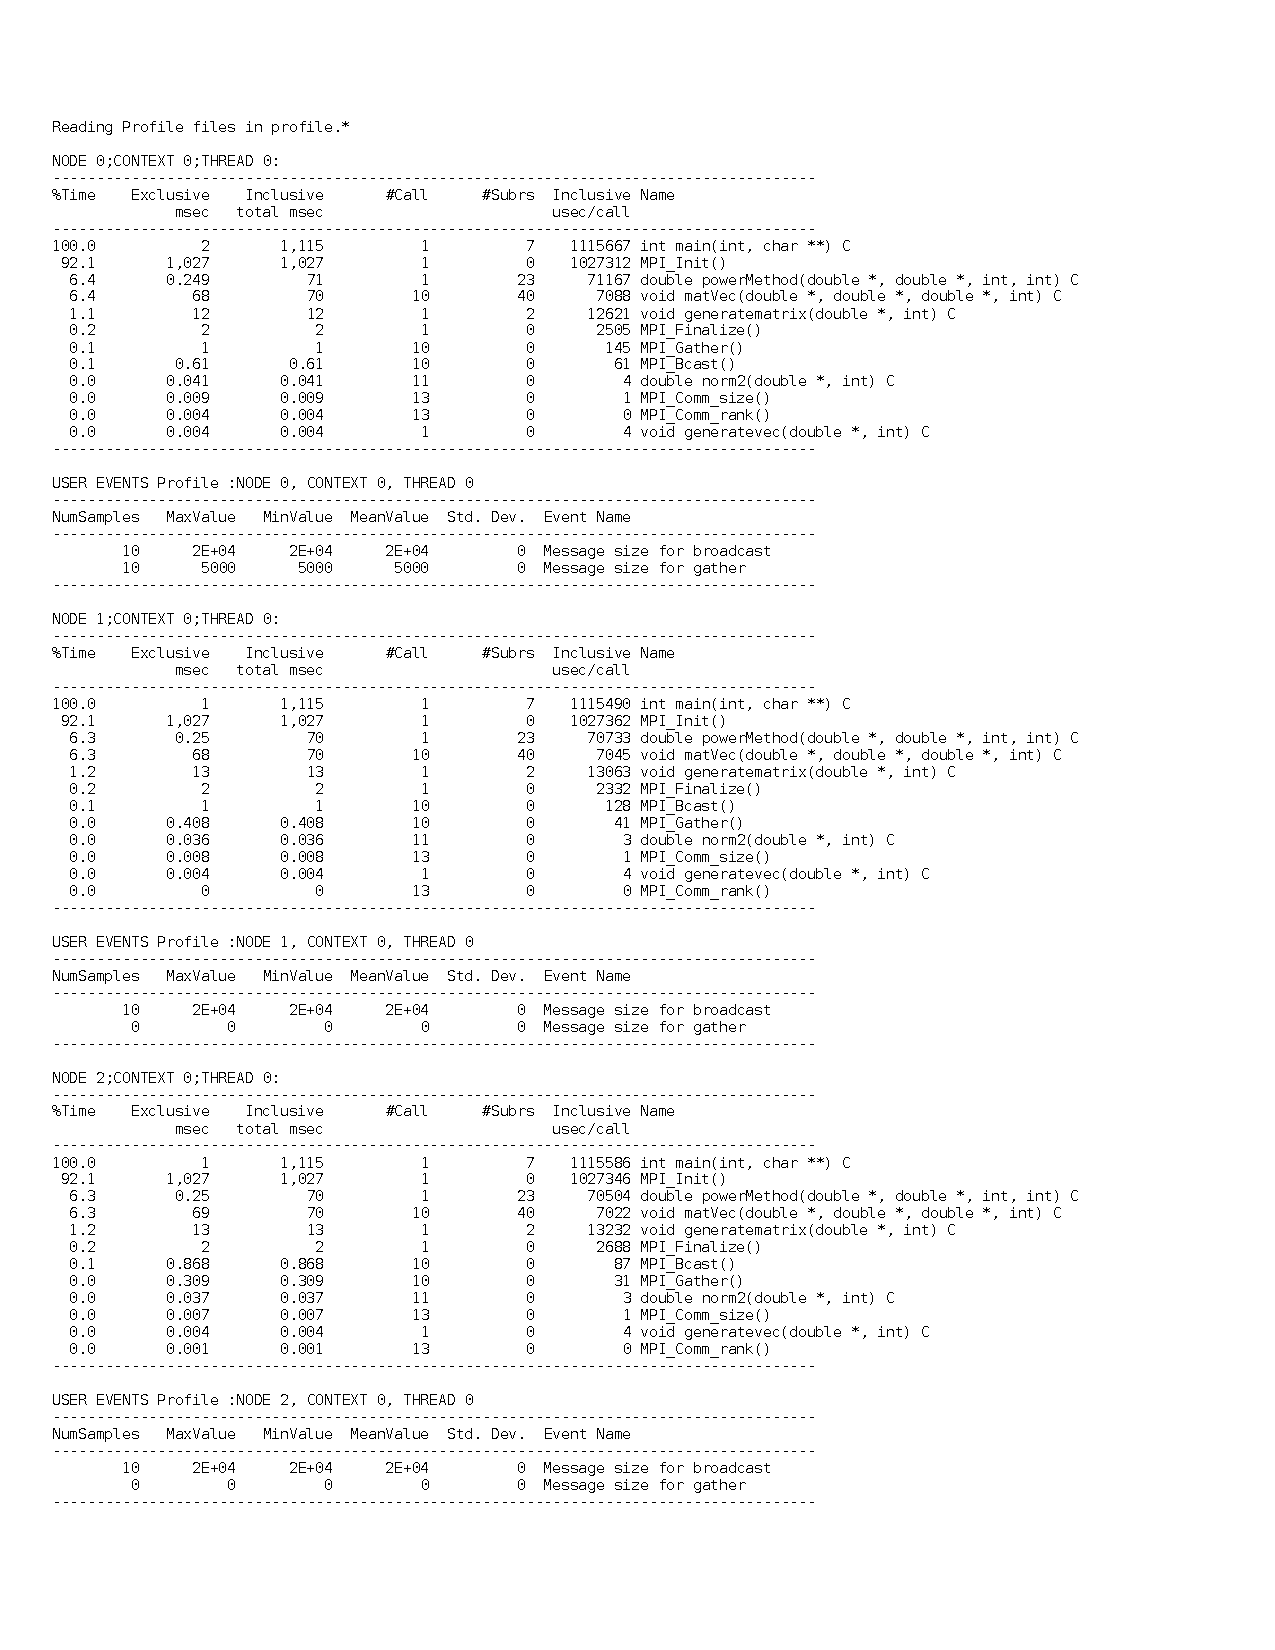
\includepdf[pages=-]{log_4.pdf}

\clearpage 
\subsection*{16 Processors}

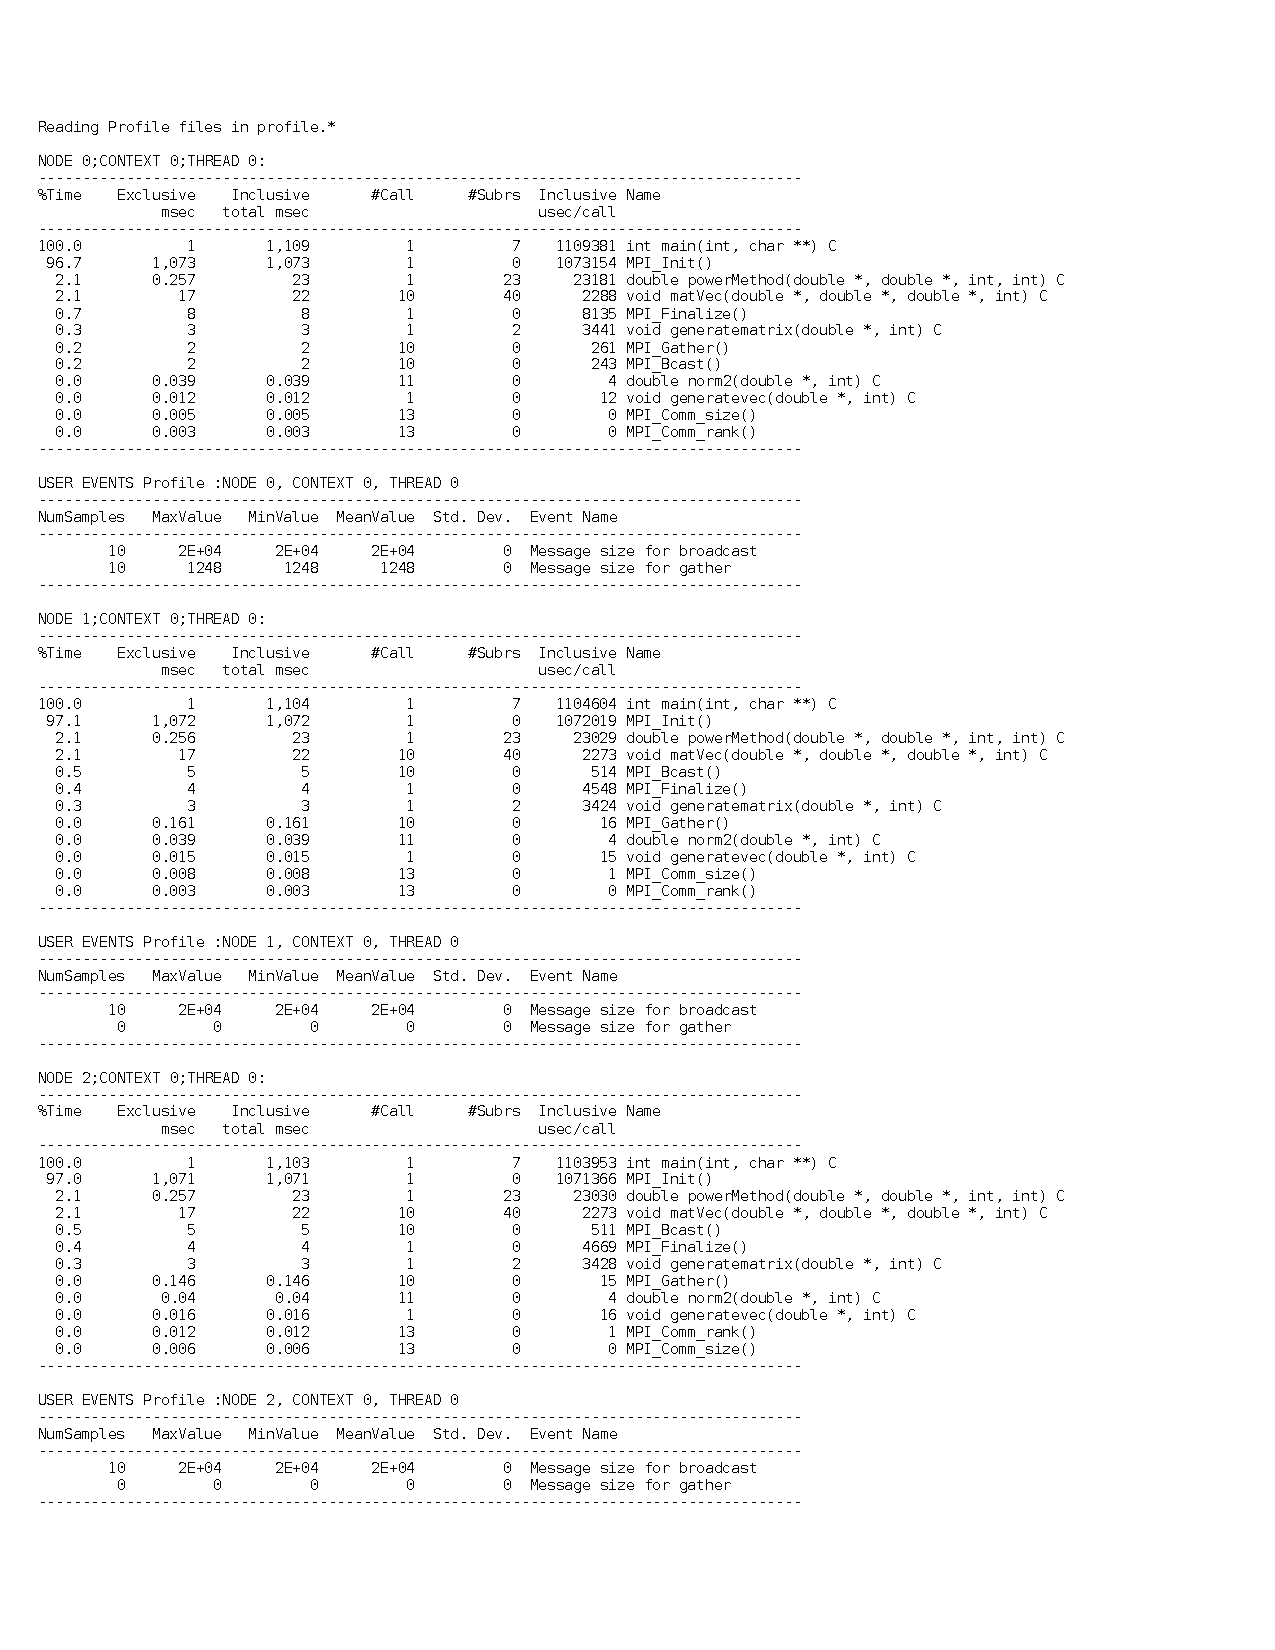
\includepdf[pages=-]{log_16.pdf}

















